%# -*- coding: utf-8-unix -*-
%%==================================================
%% chapter0.tex for SJTU Master Thesis
%%==================================================


\chapter{绪论}
\label{chapter:Introduction}

\section{研究背景和意义}
随着我国经济的飞速发展和国民生活水平的提高,人们不再只关注于温饱问题,更加追求生活质量,更加关注食品的品质、安全、营养和多样\supercite{FengZhiming2007,ZhaoQiguo2011}。随之而来的,农业生产在不断扩大生产总量的同时也需要不断升级产业结构,以提供更加安全和高品质农副产品。

然而我国目前的总体农业生产技术水平落后,现代化和信息化程度较低。农村的城镇化发展致使我国可用耕地面积逐渐减少,农村劳动人口大量涌入城镇\supercite{YuJunli2001},务农人员急剧减少,农业生产人员逐步呈现老龄化和副业化趋势\supercite{LuoChaobin2005},传统的农业生产模式已经难以维持下去,这必然会导致农业生产者对农药、化肥的过量使用,食品安全和生产环境受到前所未有的挑战,这与人民日益增长的对高品质安全食品的需求及可持续发展产生了难以消除的矛盾。同时随着中国市场的不断开放,国内农产品市场与国际市场的竞争也在不断加剧。另一方面,我国还存在水资源紧缺、幅员辽阔但可用农业土地较少、生产能耗较高、基础设施建设不完善等问题。

为了解决这一系列问题,“十三五规划”提出要推进农业现代化,转变农业发展方式,着重提出要推进农业物联网应用,提高农业信息化、智能化和精准化水平。

实现现代化的设施农业是推进农业现代化发展的重要途径\supercite{LiuLei2013}。温室作为设施农业的重要组成部分,可以减少自然环境对于农业生产的限制,合理高效利用生产资源,通过人工的方式创造适宜的农业生产环境,提高农作物产量和质量,提高农业生产集约化水平。但是目前国内温室大多停留在电气化及以下水平,依靠农业生产者的经验对温室环境进行人工控制或电气化控制。已经实现的温室自动化监控系统多为本地监控,智能化和网络化程度较低,农业生产人员需要到现场才能获取相关数据,不便于生产应用和科学研究\supercite{ZhouDele2013}。随着技术的发展进步,农业物联网为温室环境监控提供了新的思路,通过物联网技术、感知控制技术、互联网技术等先进的技术手段的综合运用可以实现基于网络的温室环境监测和控制,从而实现温室的科学管理\supercite{ZhouChunsong2014,ZhongHuahui2011,HeFen2007}。基于农业物联网的智能温室可实现远程监测温室环境,并根据作物的环境需求实施精准的温室控制,是农业物联网研究的热点\supercite{ZhaoJing2010,QiaoXiaojun2005} 。

随着近年来物联网技术、网络技术、云服务和智能终端的快速进步,使基于物联网的智能温室监测与控制成为可能。但是农业生产面积大、投入成本有限、基础设施不完善、环境比较恶劣、不易值守,与传统物联网相比有其特殊的需求,需要对其感知控制层和网络传输层部分进行特殊的设计。同时由于温室内环境是一个流场、温度场、湿度场等多个物理场耦合在一起的多输入多输出的复杂大时延系统,对于温室的精准控制和监测需要借助计算流体动力学(Computational Fluid Dynamics,CFD)对温室环境的分布和变化过程进行分析。

本文综合运用物联网技术、无线网络技术和CFD仿真技术等多领域前沿技术,设计并实现了基于农业物联网的智能温室监测与控制系统,该系统可远程监测和控制温室环境,让农业生产管理人员足不出户即可远程查看当前温室内的环境数据,通过视频查看当前温室内的实时情况,同时可通过远程操作温室内的作动器实现对温室内环境参数的控制。该系统还可结合种植作物的需求和当前温室内的实时环境,根据经过已验证的温室CFD仿真模型和机器学习模型优化的智能化温室自动控制策略,实施精准的温室环境控制,从而科学高效的管理温室。消费者也可通过该系统了解到农作物的生产环境,一方面可以让消费者吃的安心放心,另一方面也可让消费者对农业生产进行监督,促进农业生产的健康发展。

\section{设施农业的国内外研究现状}
	\subsection{国内研究现状}
进入21世纪以来,我国的温室栽培技术得到快速提升,温室总面积不断增加,占据世界温室总面积的85\%以上,是温室栽培第一生产大国\supercite{GuoShirong2012ZGSC} 。
	
我国在现代温室方面的研究开始于20世纪30年代,日光温室首先在辽宁省应用于栽培蔬菜,随后我国从日本引进塑料薄膜技术开始中小拱棚的栽培,之后我国的温室一直处于发展缓慢的小规模低水平状态,直到上世纪70年代末,随着一批国外先进设施农业技术的引入,我国的设施农业展开了新的篇章\supercite{ZhouChangji2010}。上世纪80年代开始,我国对温室环境监控系统开展研究,并开始引入计算机控制,温室环境的控制效果有了明显的改善\supercite{HanYi2016}。上世纪90年代后,通过对国外先进技术的吸收消化,我国开始自主研制温室环境监控系统。上海交通大学、中国农业大学、中科院、农科院等科研院所和高校都研制出了具有不同特点的温室监控系统。

经过多年的研究和实践,我国在现代温室方面的水平已经有了很大程度上的提高,但是在很多方面仍然落后于国际领先水平,主要体现在基础研究薄弱、设施结构不合理、装备和调控能力差、信息化和集约化程度低等方面\supercite{ZhangZhen2015,JiangWeijie2015},在温室环境的精准化、智能化监控等方面有较大的发展空间。

	\subsection{国外研究现状}
美国、日本、荷兰等发达国家对于现代温室技术的研究起步较早,发展到今天,已经将计算机监控系统大规模应用到温室自动化生产中,在设施装备、环境调控和栽培技术等方面都处于国际领先水平。
	
西欧是世界现代温室的发源地,虽然西欧国家的设施农业面积在世界总面积中占比不高,但是其现代化水平、生产质量和产量都非常高\supercite{GuoShirong2012NJNY} 。荷兰是其中比较典型的设施农业非常发达的国家之一,主要对花卉和蔬菜进行专业化集约化生产,且出口量都为世界首位,有“欧洲菜园子”之称,其温室主要以玻璃温室为主,在世界玻璃温室总面积中占比26\%以上\supercite{Watson2010,JiHong2007},农业生产的自动化程度很高,且效率很高,位居世界第一\supercite{QinLiu2015},其温室配套设备在满足内需的同时还能够出口很多到国外\supercite{Tavoletti2008}。

美国的温室主要为大型玻璃温室,现代化程度非常高。美国是最早将计算机技术投入到温室生产管理中的国家,通过政府的大力支持,采取了一系列的优惠政策,为农业现代化和信息化的发展创造了良好的氛围和环境。目前,美国约有82\%的温室环境通过计算机进行控制,27\%的农民还运用了网络技术\supercite{Kacira2011}。这样虽然提高了生产成本,但是也极大程度上给农业生产者带来了良好的经济效益\supercite{GuoShirong2012NJNY}。

以色列是典型的中东国家,气候干旱,水资源匮乏,但是以色列的设施农业却非常发达,创造了沙漠中的片片绿洲,其开发的节水灌溉系统引入了计算机控制,可以精准控制水肥比例,处于世界领先水平,此外以色列对于作物生长机理的研究也比较深入,可据此建立合理的温室控制策略\supercite{GuoShirong2012NJNY,TangLibiao2003} ,主要生产高质量的花卉和果蔬,不仅可以自给自足还大量出口国外,享有“欧洲厨房”的美誉\supercite{QinLiu2015} 。

日本是一个资源非常匮乏的国家,且人口密度非常大,因此日本大力发展集约化、自动化的设施农业,主要生产果蔬和花卉,且依赖程度非常高\supercite{YangChunjun2010} 。日本最早提出植物工厂的概念,突破了土地和环境的限制,利用先进的技术手段可以实现作物的全年不中断生产,对于世界农业发展有着重要的现实意义\supercite{HuYongguang2002} 。

由此可见,发达国家在设施农业和现代化温室方面的研究处于非常明显的领先地位,在温室管理中大面积引入计算机控制,自动化和集约化水平都较高,目前正在向更为先进的智能化、精准化和网络化的方向发展。

\section{农业物联网简介}
	\subsection{物联网概念}
1995年,比尔·盖茨在《The Road Ahead》中最早提及了Internet of Things一词\supercite{BillGate1995} ,但是受限于当时的网络技术、传感器技术和智能硬件技术的发展,并没有引起广泛的关注和重视\supercite{HeYong2016} 。2005年国际电信联盟(International Telecommunication Union,ITU)在《ITU Internet Report 2005: The Internet of Things》中正式提出了“物联网”的概念\supercite{HeYong2016,ITU2005} 。

	\begin{figure}[!htbp]
  		\centering
 		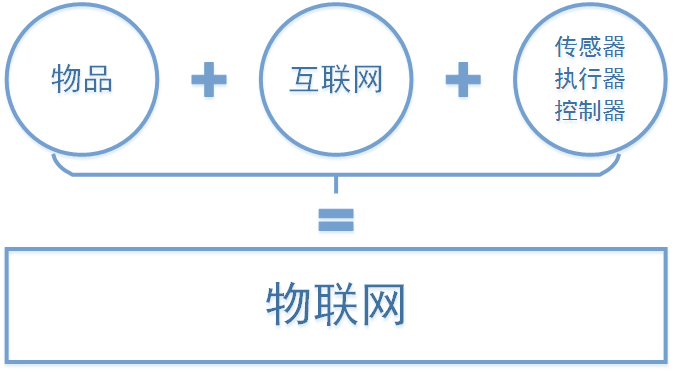
\includegraphics[width=0.5\textwidth]{01CompositionIoT.png}
  		\bicaption[fig:CompositionIoT]{物联网的基本构成}{物联网的基本构成}{Fig}{The basic composition of the Internet of Things}
	\end{figure}
为了解释物联网这一概念,首先要了解这个词是如何被创造的,物联网之父Kevin Ashton曾指出,互联网中的大部分数据都是通过人为的控制进入系统中的,在系统中,人所充当的角色无非是一种效率低下、易出错、对数据的数量和质量有所限制的路由器,并在一定的情况下可以对数据进行解释和修正,但是从另一个角度如果系统能够抛开人的限制直接连接到互联网,通过传感器获取现实世界的数据并对现实世界进行一定的控制,这样会变得更加高效、丰富和准确。物联网也即是万物相连的互联网,我们连接物体所获得的一切都是由互联网和物体自身控制,而非人\supercite{Peter2015} 。因此,物联网是建立在互联网的基础之上的,是互联网的延伸和拓展,而信息的获取和交换从人为控制扩展到了物和物之间自主进行。我们可以用一个非常简单的组成关系来描述物联网的基本构成,如\ref{fig:CompositionIoT}所示。
	
	\subsection{物联网的特征及内涵}
根据物联网的概念、物联网和互联网的异同,结合国内外专家的解释,物联网具有如下的特征和内涵:
	\begin{enumerate}
  		\item 物联网系统中包含大量各式各样的传感器,它们都担任着连接万物的使命,连续不断的获取和更新外界的实时数据。
  		\item 物联网并不是一种全新的信息传递网络,其通过各种有线或者无线网络接入互联网进行物体信息的实时传递,实现世间万物包括人之间的实时交互,最终达到为人服务的目的。
  		\item 物联网自身也是一个智能系统,它不仅可以通过传感器获取数据,同样也具备智能分析处理的能力,对数据进行清洗筛选得到有意义的数据,然后通过控制器和执行器对物体进行智能控制。
  		\item 物联网即是未来的互联网。我们希望实现的不仅仅是物与物的局部信息传递,而是最终要实现所有的人和世间万物的互连互通,这也与未来的互联网的发展趋势是一致的。
	\end{enumerate}
	
	\subsection{物联网在农业中的应用}
“十三五”规划纲要指出要加速新一代的信息基础设施建设,推进信息网络技术广泛运用,形成万物互联、人机交互、天地一体的网络空间,加快物联网基础的布局,将物联网应用在社会生活的各个方面。同时指出要推进农业现代化建设,推进农业物联网和农业大数据的实践应用,提高农业生产的智能化和精准化水平。随着物联网技术的不断发展,农业的现代化、智能化和信息化发展迎来了新的解决方案和发展机遇。
	
目前,物联网技术在工业领域已经得到了较为广泛的应用,但是农业领域的物联网应用还处在研究发展阶段。近年来,欧美等发达国家陆续开展了农业物联网的相关工作研究,并进行了一系列的实践推广,推动了农业物联网的发展。我国也在农业物联网相关方面开展了积极的研究工作,主要实现农业生产环境资源的信息互通共享,以及农产品生产和物流等过程中的信息采集和通信,形成产前合理规划提高资源利用率,产中现代化管理提高生产效率、安全生产、节约成本、提高效益,产后高效流通和安全溯源的农业物联网一条龙解决方案,但是产品多处于试验阶段,产品的稳定性、可靠性、低功耗等性能参数上与国际领先的产品还存在一定的差距。因此我国的农业物联网相关研究工作还有很大的发展空间\supercite{ChenWei2013} 。
	
	\subsection{农业物联网的特点}
农业的生产环境和工业环境相比,有其自身的特点和限制,这也决定了农业物联网所处的物理环境和网络条件与工业物联网有着本质的区别。因此农业物联网有其自己的特点和特殊需求,主要有如下几点:
	\begin{enumerate}
  			\item 成本有限,布点稀疏。农业生产的单位收益不高,投入成本有限,此外,大面积在农业生产环境内布置传感器测点会给农业作业,尤其是农业机械化作业带来干扰,这就决定了农业物联网中不可能密集布置传感器测点。因此,农业物联网在农业生产环境中应用时,往往布置稀疏的传感器测点。这就要求农业物联网具有远距离传输和灵活扩展的能力。
  			\item 环境复杂,不易值守。农业物联网工作环境往往面积较大且地形复杂,不易于值守,也无市电供电。因此,在要求各节点具有远距离传输能力的同时还要求功耗尽量小,能够依靠环境能源实现长期不间断的工作。
  			\item 环境恶劣,易受干扰。农业生产环境恶劣,设备经常长时间工作在高温、高湿、低温等极端环境下,且在进行无线通信时易受作物植被的干扰,这就对农业物联网设备的稳定性、可靠性、自诊断和免维护能力提出了要求。
  			\item 实时性要求相对较低。相比工业生产,农业环境变化缓慢,因此农业生产实时性要求不高。
	\end{enumerate}


\section{论文的主要内容与章节安排}
	\subsection{研究内容和创新点}
本文结合农业物联网技术和计算流体动力学仿真技术,对温室智能化监测与控制系统展开研究,主要有以下五部分内容:
		\begin{enumerate}
			\item 基于农业物联网的智能温室架构方案设计提出。
			\item 智能温室监测与控制系统的硬件与软件设计和实现。
			\item 针对温室机械通风三维全尺度瞬态及稳态计算流体动力学仿真模型。
			\item 针对南方地区典型的连栋塑料温室夏季机械通风实验与温室仿真模型验证。
			\item 基于温室机械通风仿真模型的传感器测点位置选择与优化,及机械通风控制策略优化设计。
		\end{enumerate}
		
相比于已有的相关研究,本文具有如下创新点:
		\begin{enumerate}
			\item 通过分析温室监控需求并参考物联网通用架构,设计提出了一种适用于温室监控的智能温室架构。设计并实现了基于该架构方案的智能温室监测与控制系统。根据农业生产的特点,构建了可灵活布点的无线传感网络,自定义了网络通信协议和流程,进行了节点低功耗设计;使用生产者消费者设计模式解决监测数据丢包;通过数据库二进制日志文件订阅解决了数据库异地同步;搭建了海量温室数据云存储系统。实现了对温室的智能感知、远程和智能控制,具有可靠性高、稳定性强、监测范围广、可灵活扩展、运行功耗低的优点。
			\item 针对南方地区典型的连栋塑料温室机械通风,建立并验证了三维全尺度瞬态及稳态计算流体动力学仿真模型,耦合了流场、温度场、湿度场等多个物理场,研究了机械通风条件下温室内的空气温度变化和分布规律。
			\item 通过仿真模型模拟了室外高温条件下的风机数量、温室长度、入口温度和环境温度变化等参数对机械通风降温效果的影响程度,并模拟了不同数量风机启闭控制的降温效果,为智能温室监测和控制系统提供了优化的夏季机械通风控制策略,有效降低了夏季温室的机械通风降温能耗,同时提供了优化的传感器测点布置策略,以少量监测点数据准确反映大型温室环境分布与变化情况。此外,还可以在温室设计阶段优化温室结构参数和设备配置。
		\end{enumerate}	
	\subsection{章节安排}
	本文的章节结构安排如下:
	
第一章,绪论。介绍了本文课题的研究背景和研究意义、国内外在设施农业和现代化温室方面的研究进展和发展趋势、农业物联网的相关内容、以及本文的主要研究内容和章节安排。

第二章,基于农业物联网的智能温室架构。分析智能温室系统在各个方面的需求,提出基于农业物联网的智能温室四层架构方案,并对每层结构进行阐述和设计。

第三章,智能温室监测与控制系统。详细介绍了基于本文农业物联网智能温室架构方案结合实际应用的具体实现,包括各层的硬件和软件实现。

第四章,温室计算流体动力学仿真及验证。基于计算流体动力学建立三维全尺度瞬态及稳态机械通风仿真模型,利用本文智能温室监测与控制系统进行机械通风实验,并通过实验结果对仿真模型进行了验证。

第五章,智能温室的实践与应用。详细介绍本文所设计实现的智能温室远程监测与控制系统在温室现场的实践与应用,以及温室仿真模型在实际应用中对于传感器测点位置选择优化作用和对温室机械通风控制策略的优化设计。

第六章,总结与展望。总结研究内容,展望研究内容的发展前景和改进方向。